\documentclass[]{article}
\usepackage[a4paper, total={6in, 10in}]{geometry}
\usepackage[utf8]{inputenc}
\usepackage{hyperref}
\usepackage{listings}
\usepackage{graphicx}
\usepackage{caption}

\begin{document}

\begin{center}
  {\large Data Mining - ID2222}\\
  \vspace{7mm}
  {\huge Homework 4\\[1ex]}
  {\Large  Graph Spectra  }\\
  \vspace{7mm}  
  {André Silva - Jérémy Navarro\\}
  \vspace{4mm}
  {\large November 30, 2020\\}
\end{center}

\section{Overview}

We chose to use \textit{Matlab} for the development of the project.\\
\\
Information about the structure of the project, as well as instructions on how to run it follow:\\
\\
\begin{lstlisting}[language=bash]
$ unzip homework4.zip
$ cd homework4/
$ matlab main.m
\end{lstlisting}\\
\\
The project is composed by:

\begin{itemize}
    \item \texttt{main.m}: The executable script which performs experimentation on the dataset.
    \item \texttt{example1.dat}: First dataset with k=4 clusters.
    \item \texttt{example2.dat}: Second dataset with k=2 clusters.
\end{itemize}

\section{Implementation}

\subsection{Read the file}

First we read the file.

\subsection{Convert edge list to adjacency matrix}

Then, we convert the graph representation from an edge list into an adjacency matrix, $A$. The diagonal in $A$ is empty.

\subsection{Construct $L=D^{-1/2}AD^{-1/2}$ }

Matrix $D$ is a diagonal matrix. For every element $d_{ii}$ the value is the sum of the row $i$ of matrix $A$.

\subsection{Eigenvector of L}

We form matrix $X$, composed, in each column, of the eigenvectors of matrix $L$.

\subsection{Normalization}

We create matrix $Y$ by normalizing $X$.

\subsection{k-clustering}

We apply K-means clustering to matrix $Y$. We consider each row as a point.

\subsection{Final clustering}

Finally, we assign each point to a cluster depending on the previous step.

\pagebreak

\section{Results}

\subsection{Clustering}

After running the algorithm on the datasets, we can extract clusters from them. In Figure \ref{fig:c1} we can see that all 4 clusters are separated. In Figure \ref{fig:c2} even if the 2 clusters are connected, we can sort every nodes in the correct cluster.

\begin{figure}[!h]
    \centering
    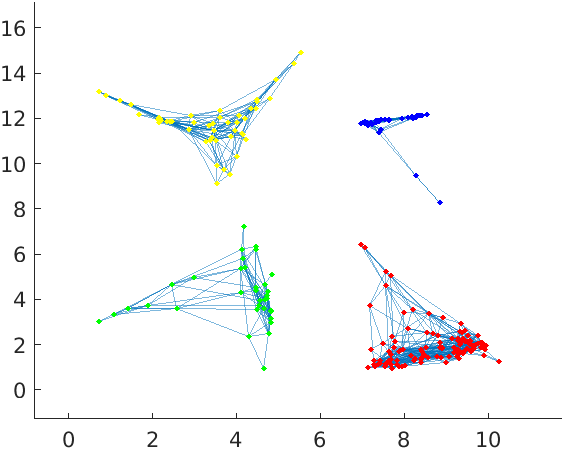
\includegraphics[width=.8\textwidth]{../example1_clusters.png}
    \caption{Dataset 1 with cluster highlighted ($k=4$)}
    \label{fig:c1}
\end{figure}

\begin{figure}[!h]
    \centering
    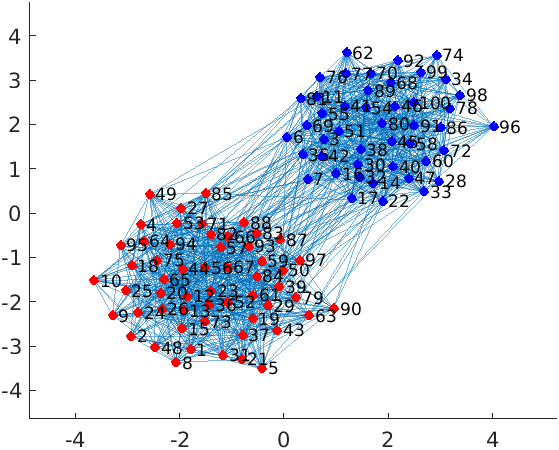
\includegraphics[width=.8\textwidth]{../example2_clusters.png}
    \caption{Dataset 2 with cluster highlighted ($k=2$)}
    \label{fig:c2}
\end{figure}

\pagebreak

\subsection{Sparsity pattern}

We can see in, Figure \ref{fig:sp1}, that when there is no connection between clusters the sparsity matrix is composed by non-overlapping blocs. However, in Figure \ref{fig:sp2} clusters are connected and highly overlap, making it hard to see two well defined blocs.


\begin{figure}[!h]
    \centering
    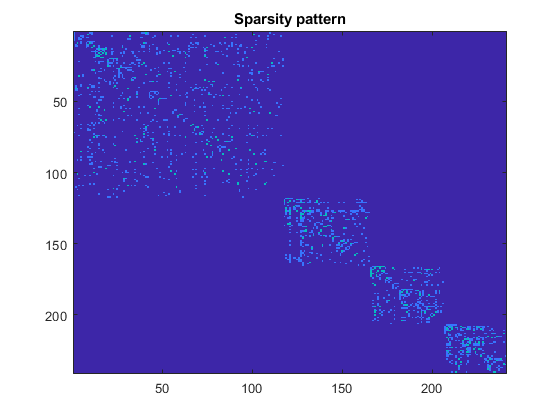
\includegraphics[width=.8\textwidth]{../example1_sparsityPattern.png}
    \caption{Sparsity pattern for dataset 1. Cluster are not connected.}
    \label{fig:sp1}
\end{figure}

\begin{figure}[!h]
    \centering
    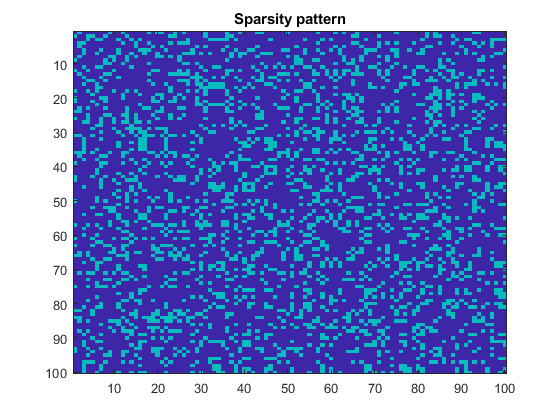
\includegraphics[width=.8\textwidth]{../example2_sparsityPattern.png}
    \caption{Sparsity pattern for dataset 2. Clusters are strongly connected.}
    \label{fig:sp2}
\end{figure}

\pagebreak

\subsection{Fiedler vector}

We visualize the fiedler vector for each of the datasets.

\begin{figure}[!h]
    \centering
    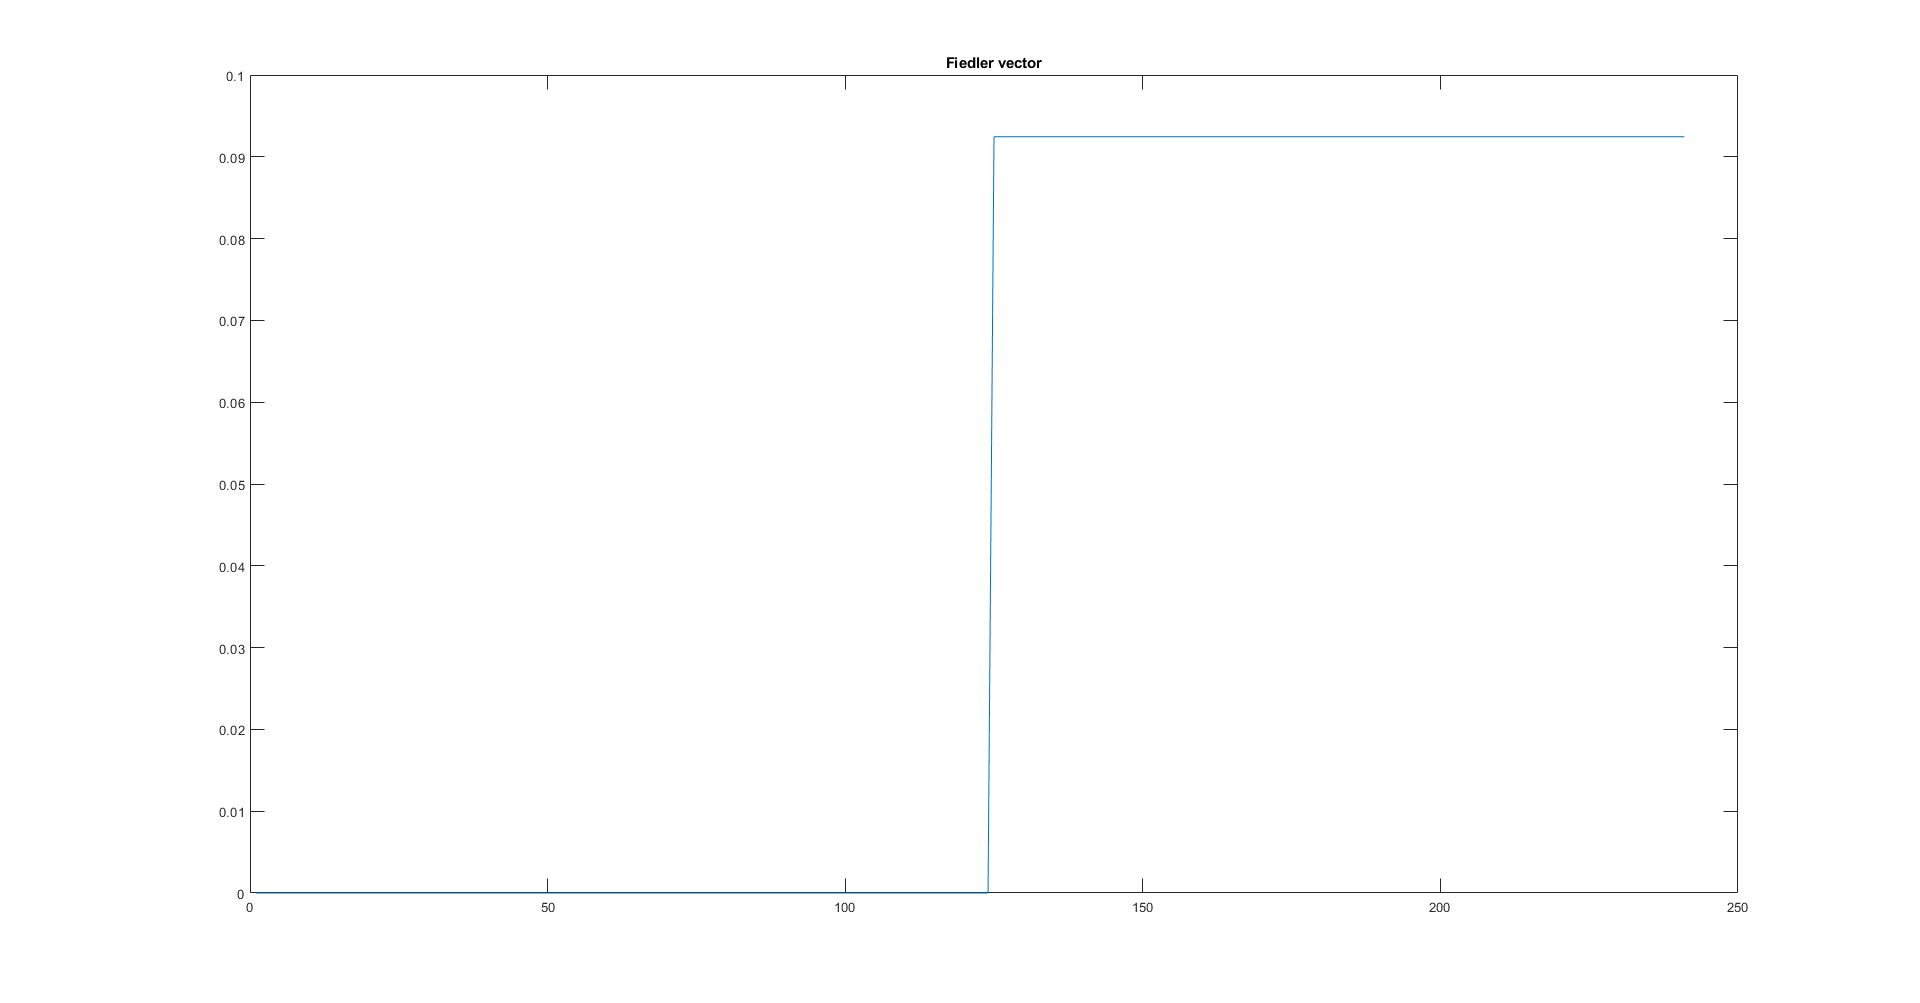
\includegraphics[width=.8\textwidth]{../example1_fielderVector_2.png}
    \caption{Fiedler vector for dataset 1}
    \label{fig:lpG1}
\end{figure}

\begin{figure}[!h]
    \centering
    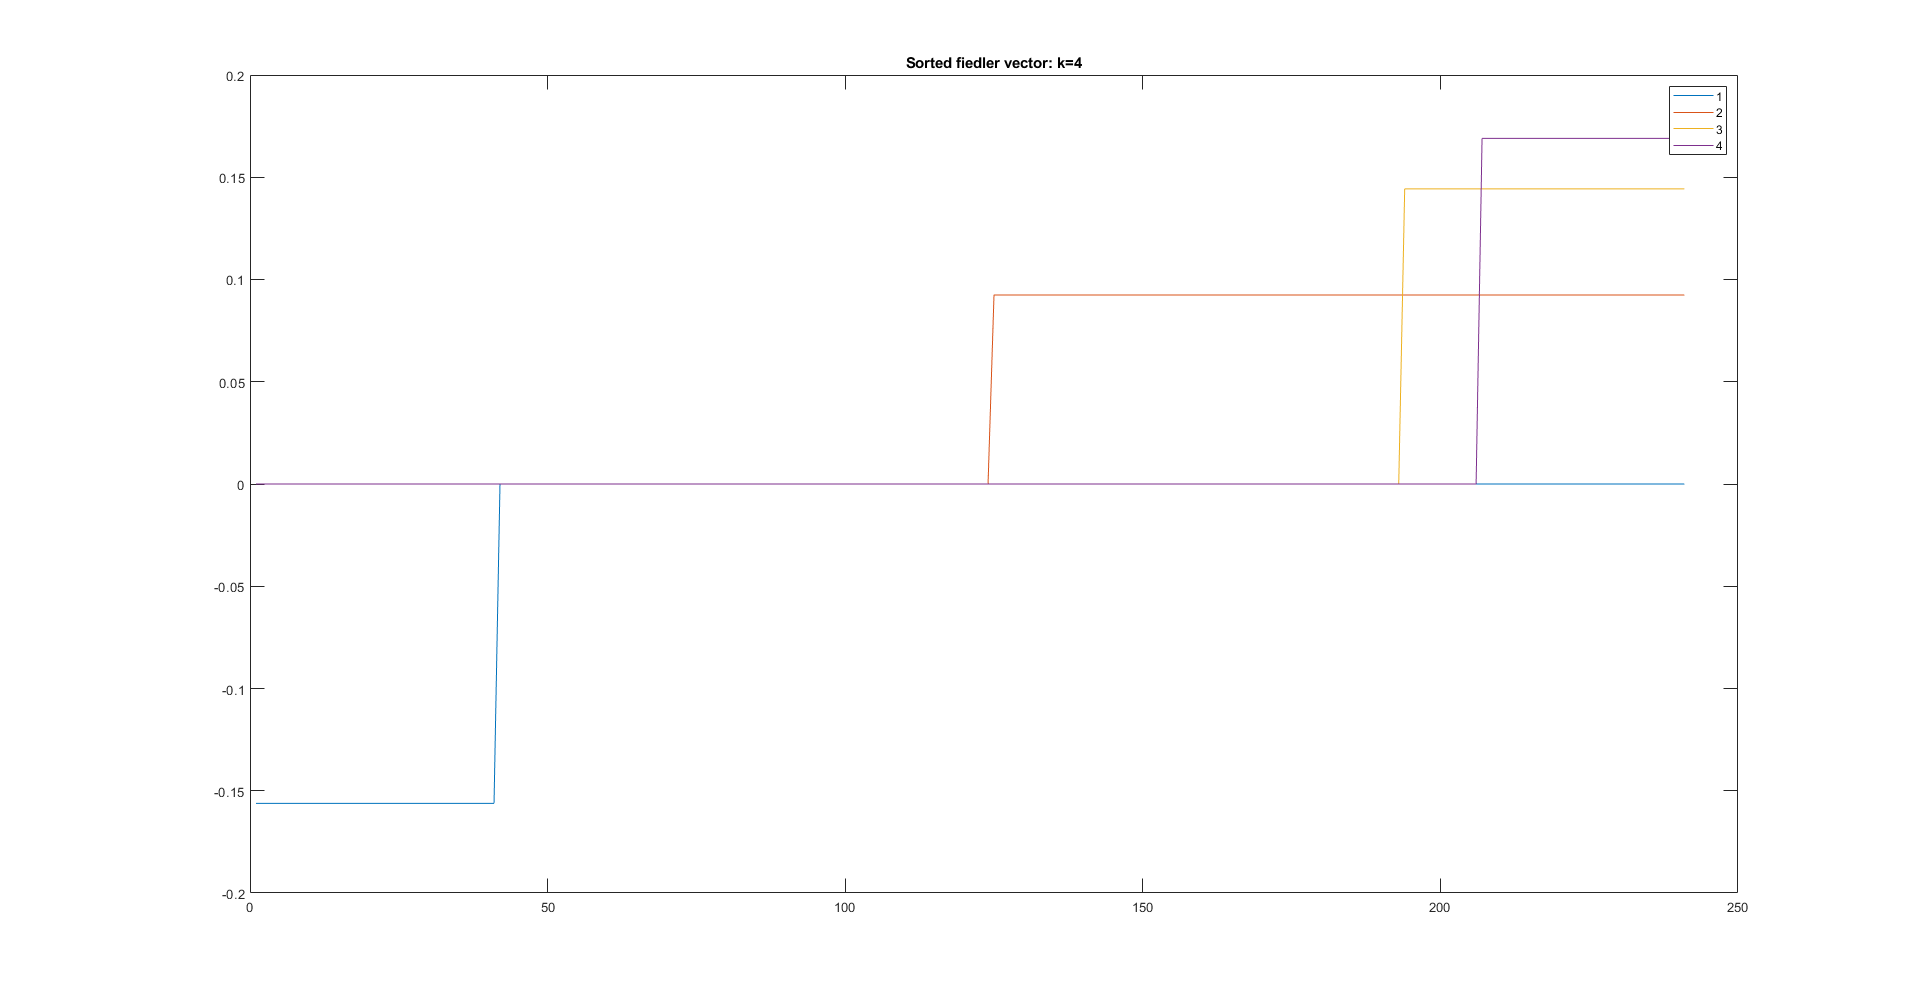
\includegraphics[width=.8\textwidth]{../example1_fielderVector.png}
    \caption{k-eigenvectors for dataset 1}
    \label{fig:lpG11}
\end{figure}

\begin{figure}[!h]
    \centering
    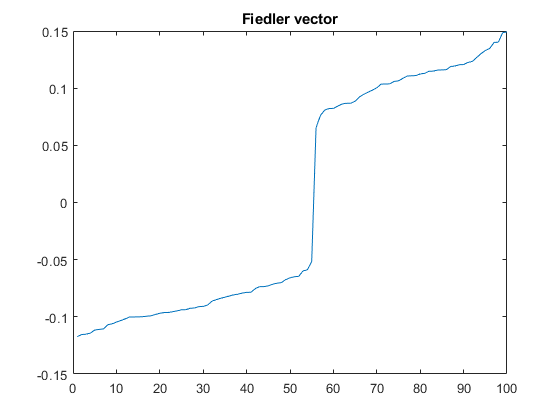
\includegraphics[width=.8\textwidth]{../example2_fielderVector_2.png}
    \caption{Fiedler vector for dataset 2}
    \label{fig:lpG2}
\end{figure}

\begin{figure}[!h]
    \centering
    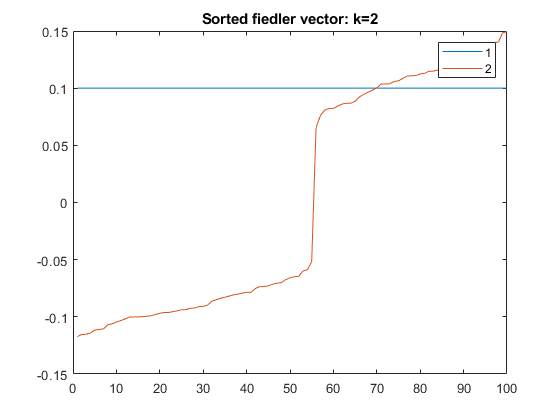
\includegraphics[width=.8\textwidth]{../example2_fielderVector.png}
    \caption{k-eigenvectors for dataset 2}
    \label{fig:lpG22}
\end{figure}


\end{document}
